\section{Problem 1}
\label{part1}
\subsection*{Question}
\begingroup
\begin{verbatim}
The "friendship paradox" (http://en.wikipedia.org/wiki/Friendship_paradox)
says that your friends have more friends than you do.  

1.  Explore the friendship paradox for your Twitter account.  Since
Twitter has directional links (i.e., "followers" and "following"),
we'll be investigating if the people you follow (Twitter calls these
people "friends") follow more people than you.  If you are following <
50 people, use my twitter account "phonedude_mln" instead of your own.

Create a graph of the number of friends (y-axis) and the friends sorted
by number of friends (x-axis).  (The friends don't need to be labeled on
the x-axis as "Bob", "Mary", etc. -- just 1, 2, 3 ...)  In other words,
if you have 100 friends your x-axis will be 1..101 (100 + you), and the
y-axis value will be number of friends that each of those friends has.
The friend with the lowest number of friends will be first and the friend
with the highest number of friends will be last.

Do include yourself in the graph and label yourself accordingly.  Compute
the mean, standard deviation, and median of the number of friends that
your friends have.

The appropriate part of the Twitter API to use is:

https://dev.twitter.com/rest/reference/get/friends/list

\end{verbatim}

\newpage
\begin{enumerate}
\item This assignment was comparatively easy when compared to the second assignment. 
\item I used twittersearch library to get 1000 URIs in second assignment, but to get the list of friends in the twitter this library is of no help.
\item So I figured tweepy does that job with out any trouble. 
\item As I already have the consumer key and tokens I used them here in order get the data. 
\item In tweepy there are these predefined functions ``friends\_count'' which will give the count of the friends whom we follow and function ``friends'' gives the list of friends for a particular user. 
\item Function ``friends'' by default gives only list of 20  friends. After a little research I figured we can set the list to a desired count.
\item My twitter account is very new so I don't have many friends so I used ``phonedude\_mln''
\item I wrote a Python program to get the list of friends and their friends.  The output(followed.txt) from this program is not sorted. 
\item So I sorted the list by using a simple command in Linux. The Linux command is as below and the result is stored in followed-sorted.txt file.
 \begin{lstlisting}[frame=single]
sort -n -k1 followed.txt > followed-sorted.txt
\end{lstlisting}
\item ``Phonedude\_mln'' had 148 friends in total. But there is an other person who have the same number of friends so when I am highlighting ``phonedude\_mln'' two bars in the bar plot got highlighted. 
\item I calculated Mean , Standard Deviation and median in R using simple commands as shown in Listing \ref{lst:q1Rscript}. 
	\begin{itemize}
		\item Mean:  404.926174496644
		\item Median:  191
		\item Standard Deviation:  545.993999248776
	\end{itemize}
\item I plotted the graph in scatter plot which can be seen Figure \ref{fig:q1-2}, but it is not as clear as the bar plot. 
\end{enumerate}
\newpage

\lstinputlisting[language=python, frame=single, caption={Python Program for printing the list of followers}, label=lst:q1python, captionpos=b, numbers=left, showspaces=false, showstringspaces=false, basicstyle=\footnotesize]{q1/getfollowers.py}
\newpage
\lstinputlisting[language=R, frame=single,breaklines=true, caption={R script for statistics and bar plot shown in Figure \ref{fig:q1-1}  }, label=lst:q1Rscript, captionpos=b, numbers=left, showspaces=false, showstringspaces=false, basicstyle=\footnotesize]{q1/barplot.R}

\begin{figure}
	 \begin{center}
		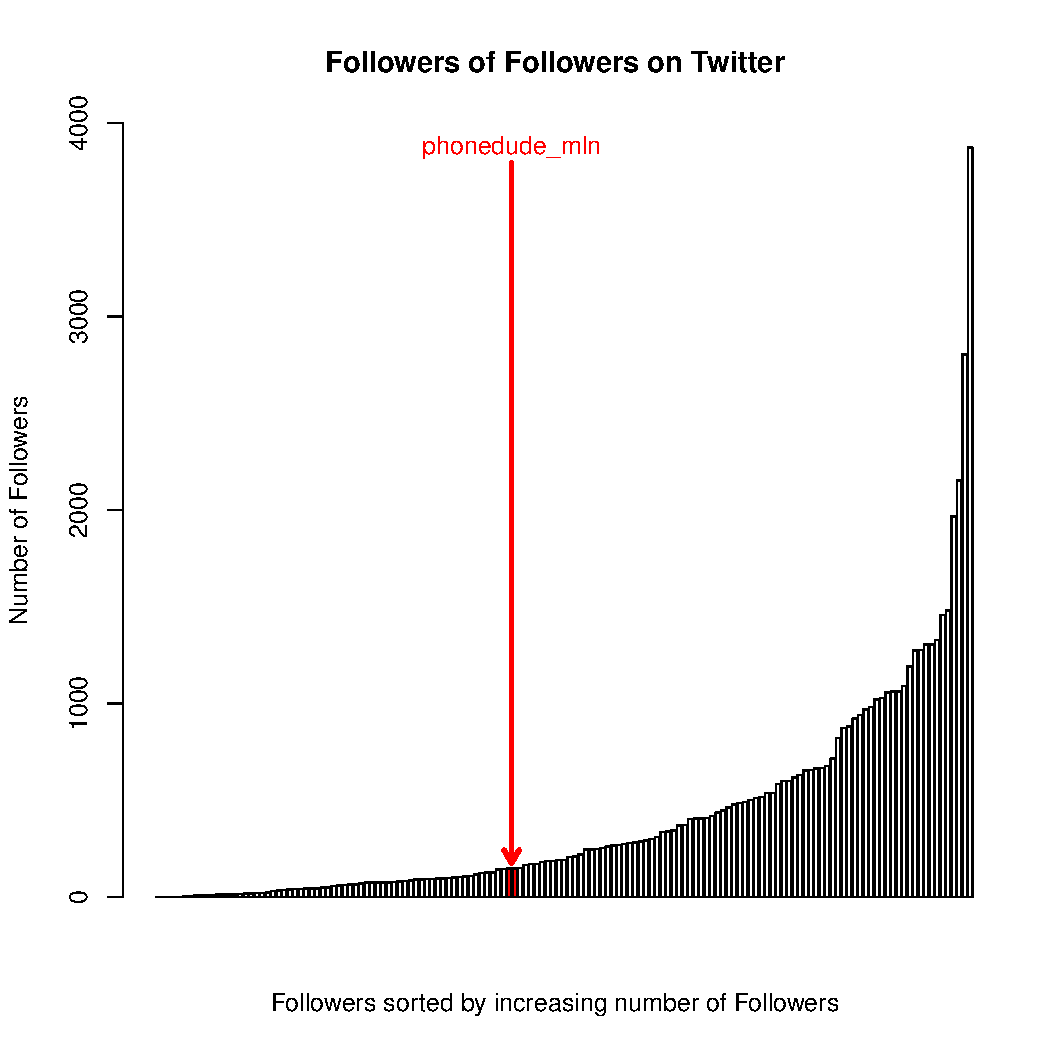
\includegraphics[scale=0.8]{q1/barplot.pdf}
		\caption{BarPlot showing the count of phonedude\_mln's Twitter follower's followers }
		\label{fig:q1-1}
 	\end{center}
\end{figure}
\begin{figure}
	 \begin{center}
		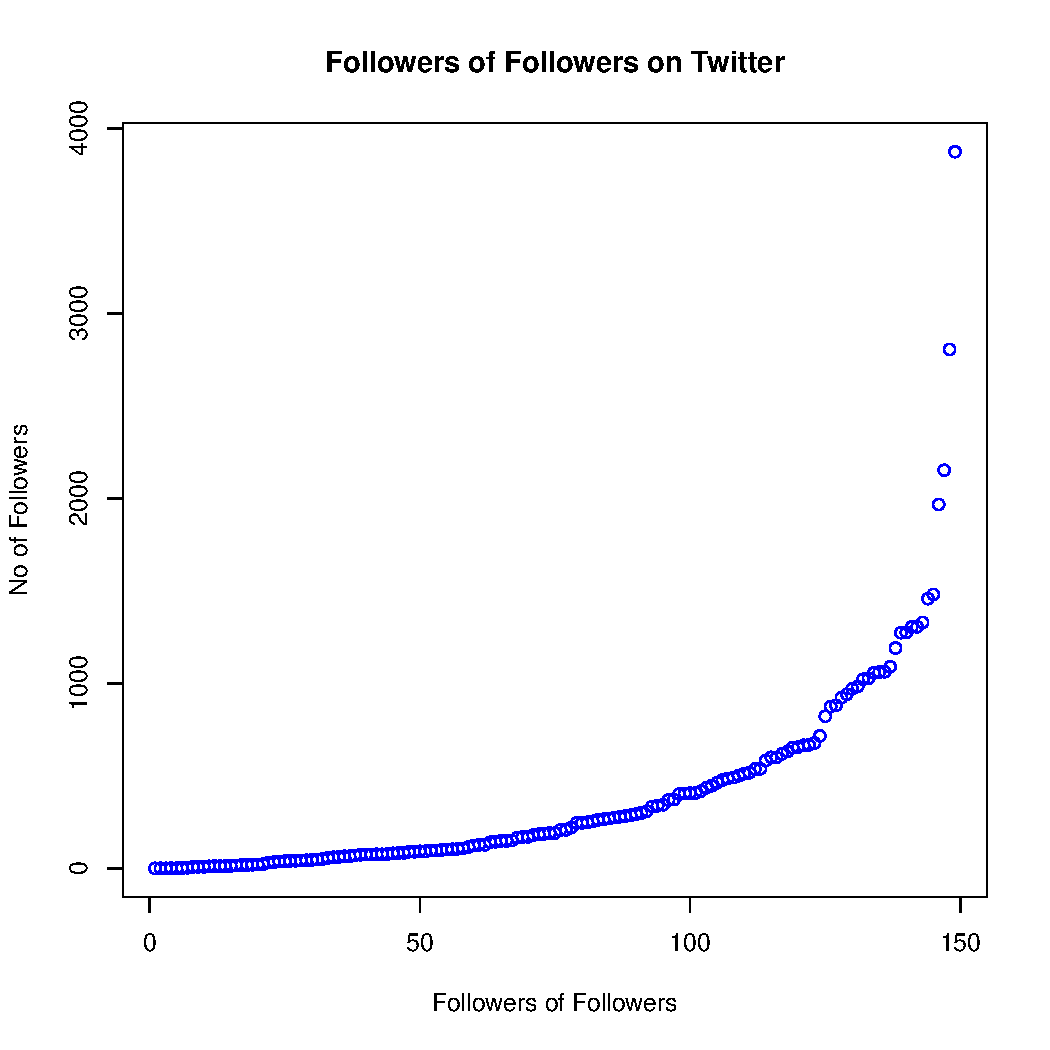
\includegraphics[scale=0.8]{q1/q1-scatterplot.pdf}
		\caption{ScatterPlot showing the count of phonedude\_mln's Twitter follower's followers }
		\label{fig:q1-2}
 	\end{center}
\end{figure}